% Final Report
% The final reports should be in the style of a short research paper of three pages (about one page text plus plots & figures).
% The format for the report has to be the standard IEEE conference format: https://www.ieee.org/conferences/publishing/templates.html

\documentclass[conference]{IEEEtran}
\usepackage{amsmath,amssymb,amsfonts}
\usepackage{algorithmic}
\usepackage{cite}
\usepackage{bm}
\usepackage{graphicx}
\usepackage{textcomp}
\usepackage{xcolor}
\usepackage[caption=false,font=footnotesize]{subfig}

% \usepackage{subcaption}
% \captionsetup{compatibility=false}


\def\BibTeX{{\rm B\kern-.05em{\sc i\kern-.025em b}\kern-.08emT\kern-.1667em\lower.7ex\hbox{E}\kern-.125emX}}


\begin{document}


\title{Neural Networks for Inverse Kinematics Problems in Robotics}

\author{\IEEEauthorblockN{Franziska Schwaiger}
    \IEEEauthorblockA{\textit{Matriculation number: 03658670}}
    \and
    \IEEEauthorblockN{Thomas Barthel Brunner}
    \IEEEauthorblockA{\textit{Matriculation number: 03675118}}
}

\maketitle

\section*{Introduction}

In our project, we are evaluating the feasibility of using neural networks for inverse kinematics problems in robotics. In this report, we outline the progress made and discuss the results we have obtained.

\section*{Methods}
\subsection*{Robot Simulations}

To train and test our models, we developed simulations of planar robotic arms with revolute joints. As we are interested in testing the limits of our models, we created simulations of arbitraty degrees of freedom (DOFs). In general, the forward kinematics equations of a planar robot arm with link lengths \( l_i \) and \( N \) revolute joints with joint angles \( \theta_i \) can be described as:
\begin{equation}
    x_{TCP} = \sum_{i=1}^{N}{l_i \cos\left( \sum_{j=1}^{i}{\theta_j} \right)}
\end{equation}
\begin{equation}
    y_{TCP} = \sum_{i=1}^{N}{l_i \sin\left( \sum_{j=1}^{i}{\theta_j} \right)}
\end{equation}
\begin{equation}
    \theta_{TCP} = \sum_{i=1}^{N}{\theta_i}
\end{equation}

These equations were modified for fast vectorized numerical computation by the element-wise computation of the sine and cosine of the matrix multiplication of the joint angles vector \( \bm{\theta} = \left[ \theta_1, \theta_2 , ... \right]^\text{T} \) with an upper triangular matrix with ones as elements \( \bm{U} \). The results are then multiplied with the link lengths vector \( \bm{l} = \left[ l_1, l_2, ... \right]^\text{T} \), as shown in Equations \ref{xtcp vectorized} and \ref{ytcp vectorized}.
\begin{equation}
    x_{TCP} = \cos \left( \bm{\theta}\ \bm{U} \right) \bm{l}
    \label{xtcp vectorized}
\end{equation}
\begin{equation}
    y_{TCP} = \sin \left( \bm{\theta}\ \bm{U} \right) \bm{l}
    \label{ytcp vectorized}
\end{equation}

In our current setup, we do not take the angle of the tool center point (TCP) into consideration. Thus, the location of the TCP is defined by its \( x, y \) coordinates. As a result of this, all simulations with more than 2 DOF can up to infinite solutions of the inverse kinematics for a given TCP position. The 2 DOF robot arm can have up to two solutions.

\subsection*{Dataset}

The dataset used for training is composed of one million samples of robot configurations for each DOF. Figure~\ref{fig:datasets} shows an illustration of the datasets. Each configuration was sampled from a normal distribution $ \theta_i \sim \mathcal{N}(\mu=0, \sigma=0.2) $. Thus, the dataset is composed mostly of configurations in which the robot arm is extended. This reflects real-world use cases of robot arms, which have limited workspaces and whose tasks are focused on one section of the workspace. Moreover, limiting the range of the joints improved the performance of the networks, as this avoids the discontinuity in the angles at \( \theta = \pi \).

% TODO add images of datasets

\subsection*{Considering Singularities}

As already mentioned in the previous section, we avoid discontinuities by restricting the configuratoin space of the robot. Yet we implemented two approaches which consider this discontinuity in the angles at \( \theta = \pi \) to generalize the implemented networks to inverse kinematics problems.

\subsubsection*{First approach}
The first approach uses a  non-minimal parameterization of ...

\subsubsection*{Second approach}




\subsection*{Conditional Variational Autoencoder}

\subsection*{Invertible Neural Networks}

Autoregressive flows ...

\subsection*{Hyperparameter Optimization}

For our tests, we trained a network for each robot simulation (DOF). Thus, the sizes and selection of hyperparameters of each network had to match the compleity of the simulation. To compare the performance of the networks across different DOFs in a fair setting, we used Tune \cite{liaw2018tune} to perform a random search of the hyperparameters. To reduce computation time, we trained the models using a subset of the main dataset, which was composed of \( 1e4 \) samples.

% TODO eventually add table with tuned parameters and 
% the range of the parameters!

\subsection*{Implementation}

The previous two model architectures (cVAE and INN) have been implemented in PyTorch and are inspired by existing implementations in  \cite{graviraja2019, freia2020}. We utilized the Google Compute Engine to train our models.

\section*{Experimental Evaluation}

\subsection*{Evaluation protocol}

We extended the DoF of the robots up to 15 DoF and performed Baysian optimization for the hyperparameters for $DoF = [4, 6, 10, 15]$. But now it is important to mention that due to HPO, the number of trainable parameters differs between cVAE and INN. 
For the cVAE, we optimized the learning rate, the weight decay, the number of hidden layers for the encoder and decoder and the amount of neurons per layer. For the INN, we optimized the learning rate, the weight decay, the number of coupling layers, the amount of layers per subnet and also the number of neurons per subnet layer. 
Both networks have been trained for 60 epochs. Both networks have been trained on a dataset with 1 million samples and a train and test spit of 70 and 30, respectively. For evaluation, we used again the two evaluation metrics  we have already described in the midterm report.

\subsection*{Results}

% In Figures ... the area of the convex hull of the 0.97 percentile of the end-effector coordinates is visualized. In the case of 100 samples, this means the value of the area which includes the 97 nearest points to the ground truth, allowing 3 outliers. The actual end point of each sample may deviate slightly from the target. Also to mention is that the convex hull of rejections sampling (eps = ...) produces a value of ....
% contour lines enclose the regions containing $97\%$ of these end points.

\begin{itemize}
	\item For evaluation, we considered discontinuities of the joint space by modifying the loss function (2st approach) 
	\item Minimal representation of joint angles, as number of DoF increases, doubling the number (1st approach) is not a good idea
	\item Because of HPO, the number of parameters over the amount of DoF differs and does not increase cosistently
	\item The INN Does a better job in estimating the full posterior of the joint configuration as the cVAE
\end{itemize}

\begin{figure}[!ht]
\centering
	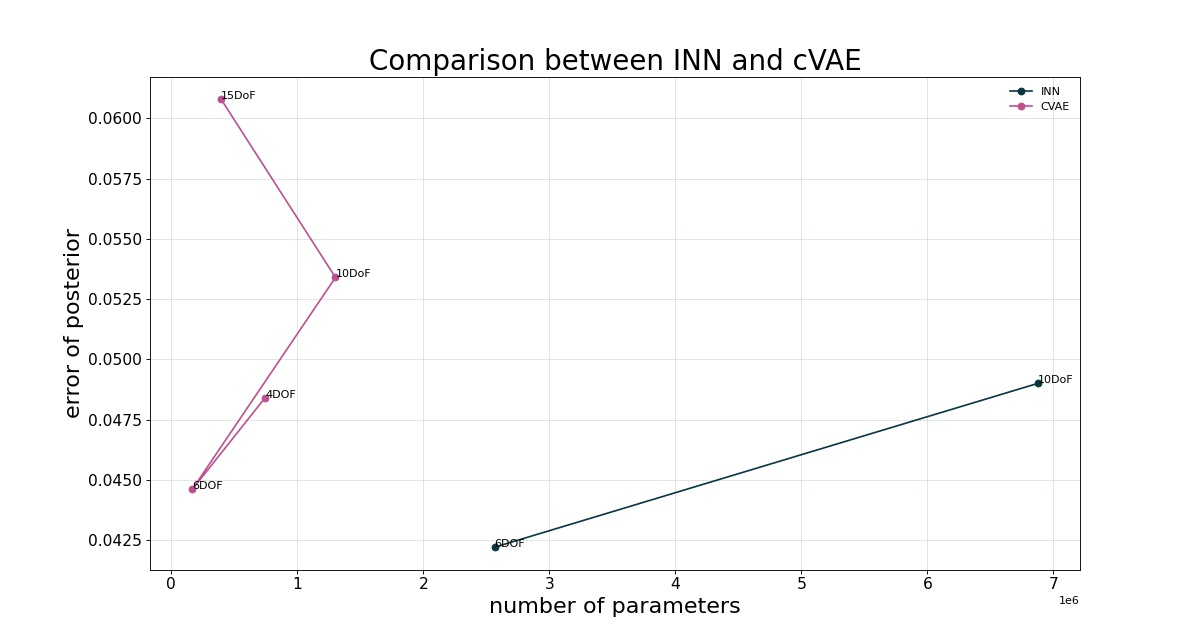
\includegraphics[width=\linewidth]{figures/comparison_e_posterior_alternative.jpg}
    \label{fig:plot:posterior}
    \caption{\label{fig:plot:posterior} Results. Mismatch of posterior. Needs to be completed.}
\end{figure}

\begin{figure}[!ht]
\centering
	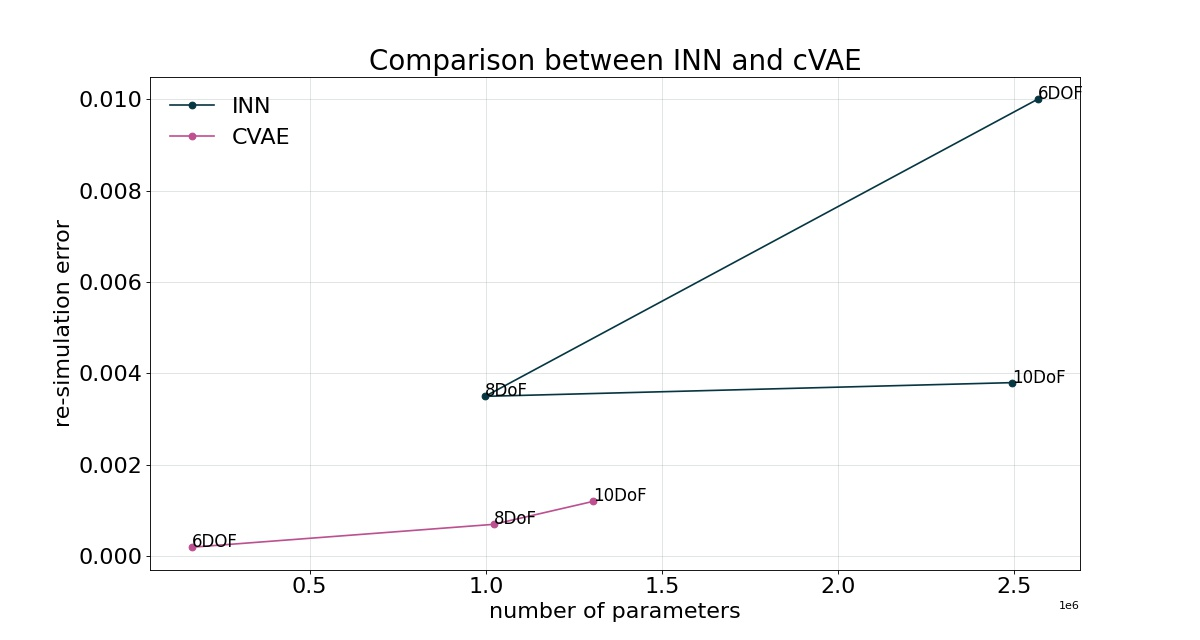
\includegraphics[width=\linewidth]{figures/comparison_e_resim_alternative.jpg}
    \label{fig:plot:posterior}
    \caption{\label{fig:plot:resim} Results. Mismatch of re-simulation error. Needs to be completed.}
\end{figure}

\begin{figure*}[tbh]
\centering
	\subfloat[Rejection Sampling]{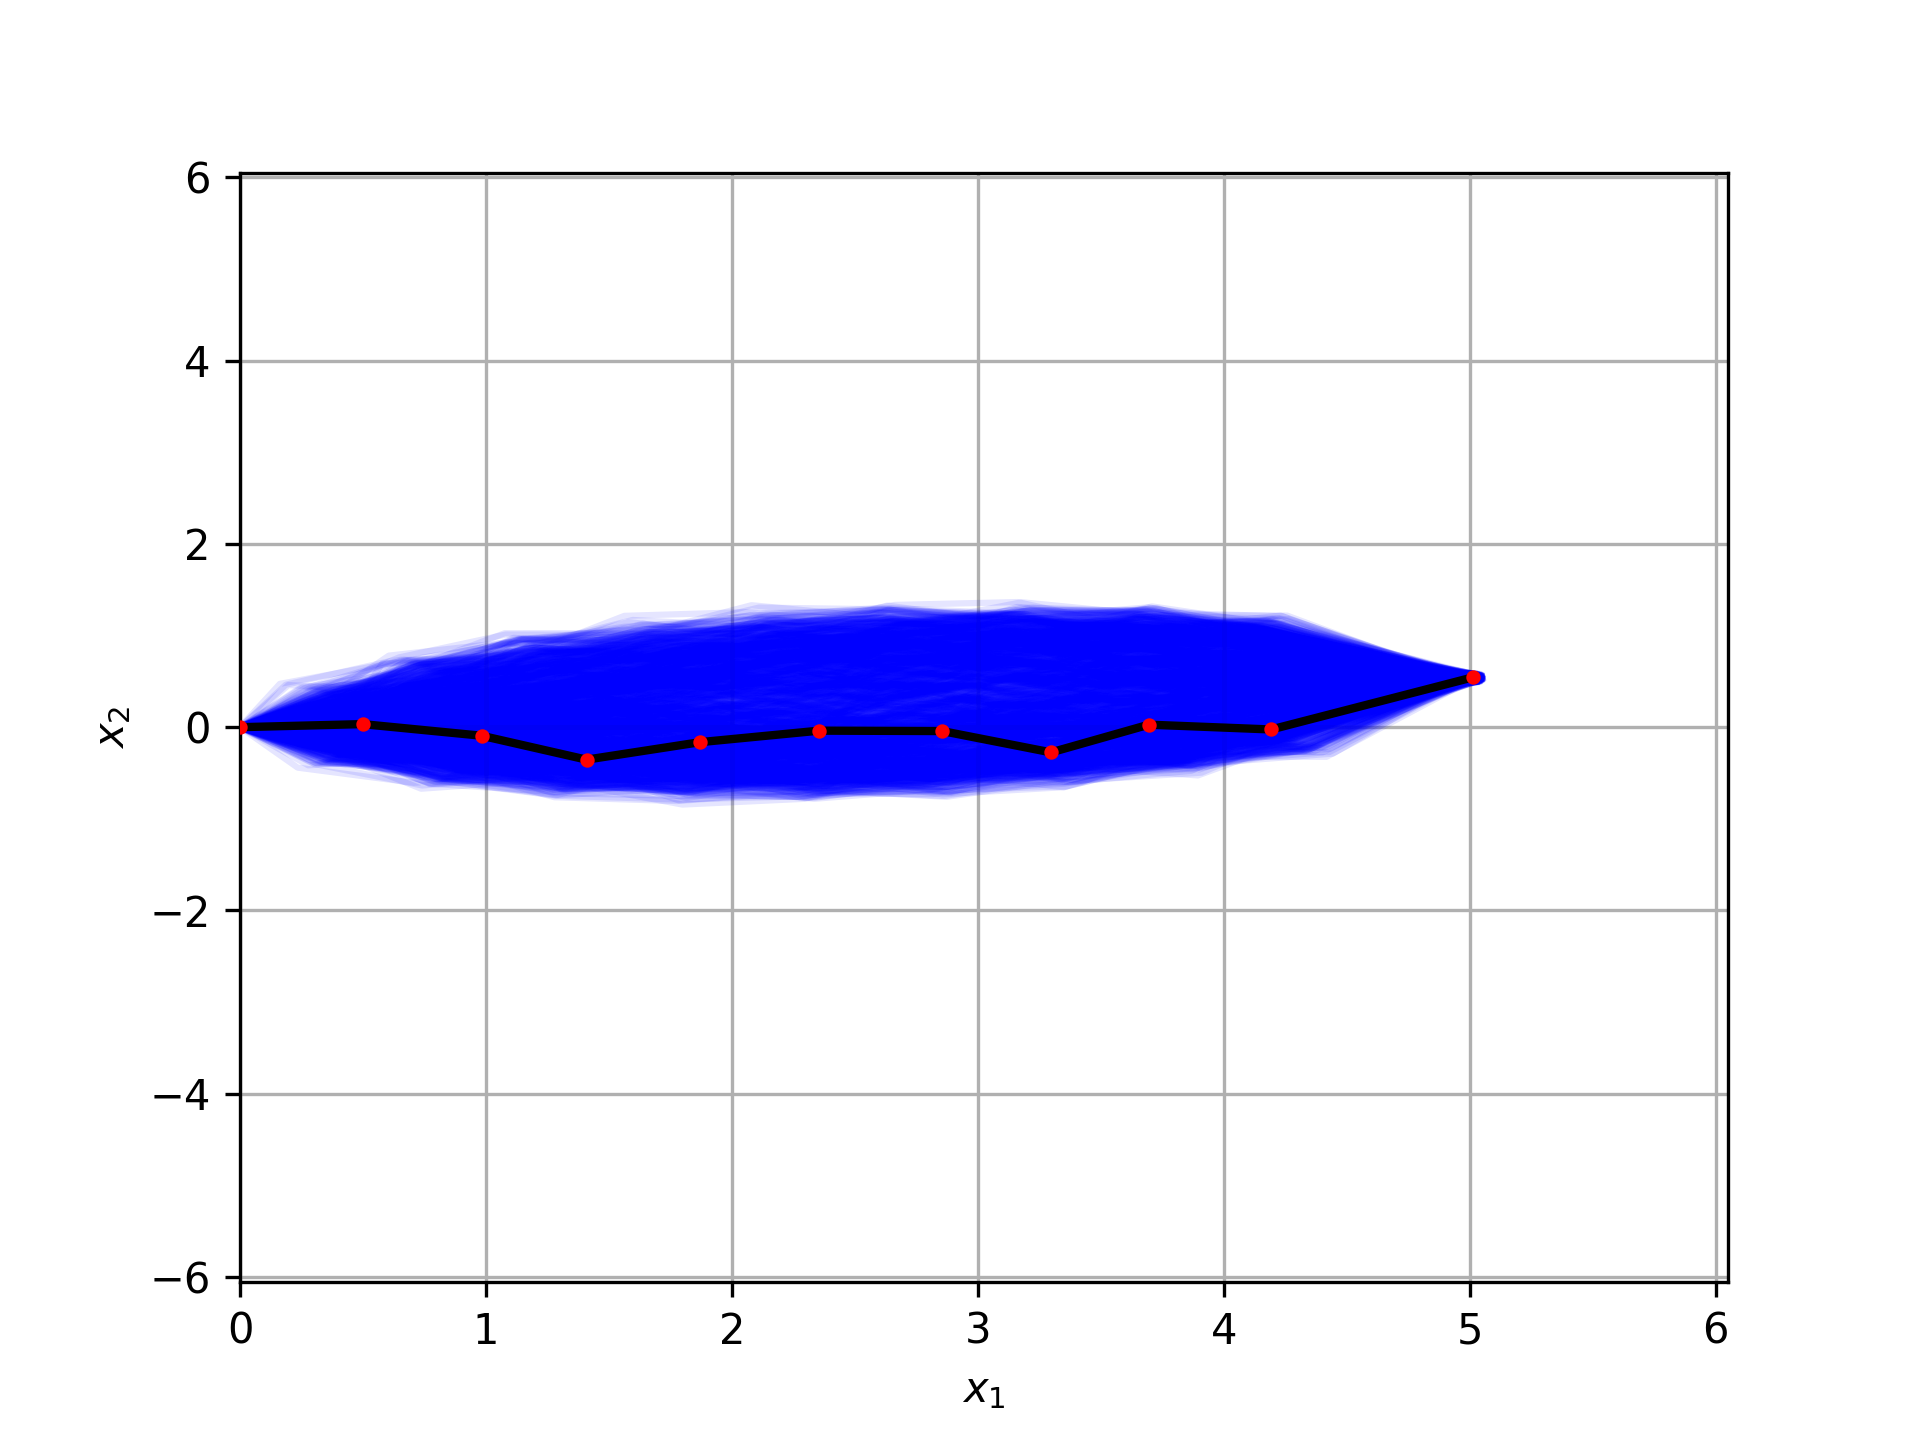
\includegraphics[width=0.29\linewidth]{figures/rejection_sampling_CVAE_10DOF.png}
    \label{fig:rejection_sampling:10DOF}}
    %
    \subfloat[cVAE]{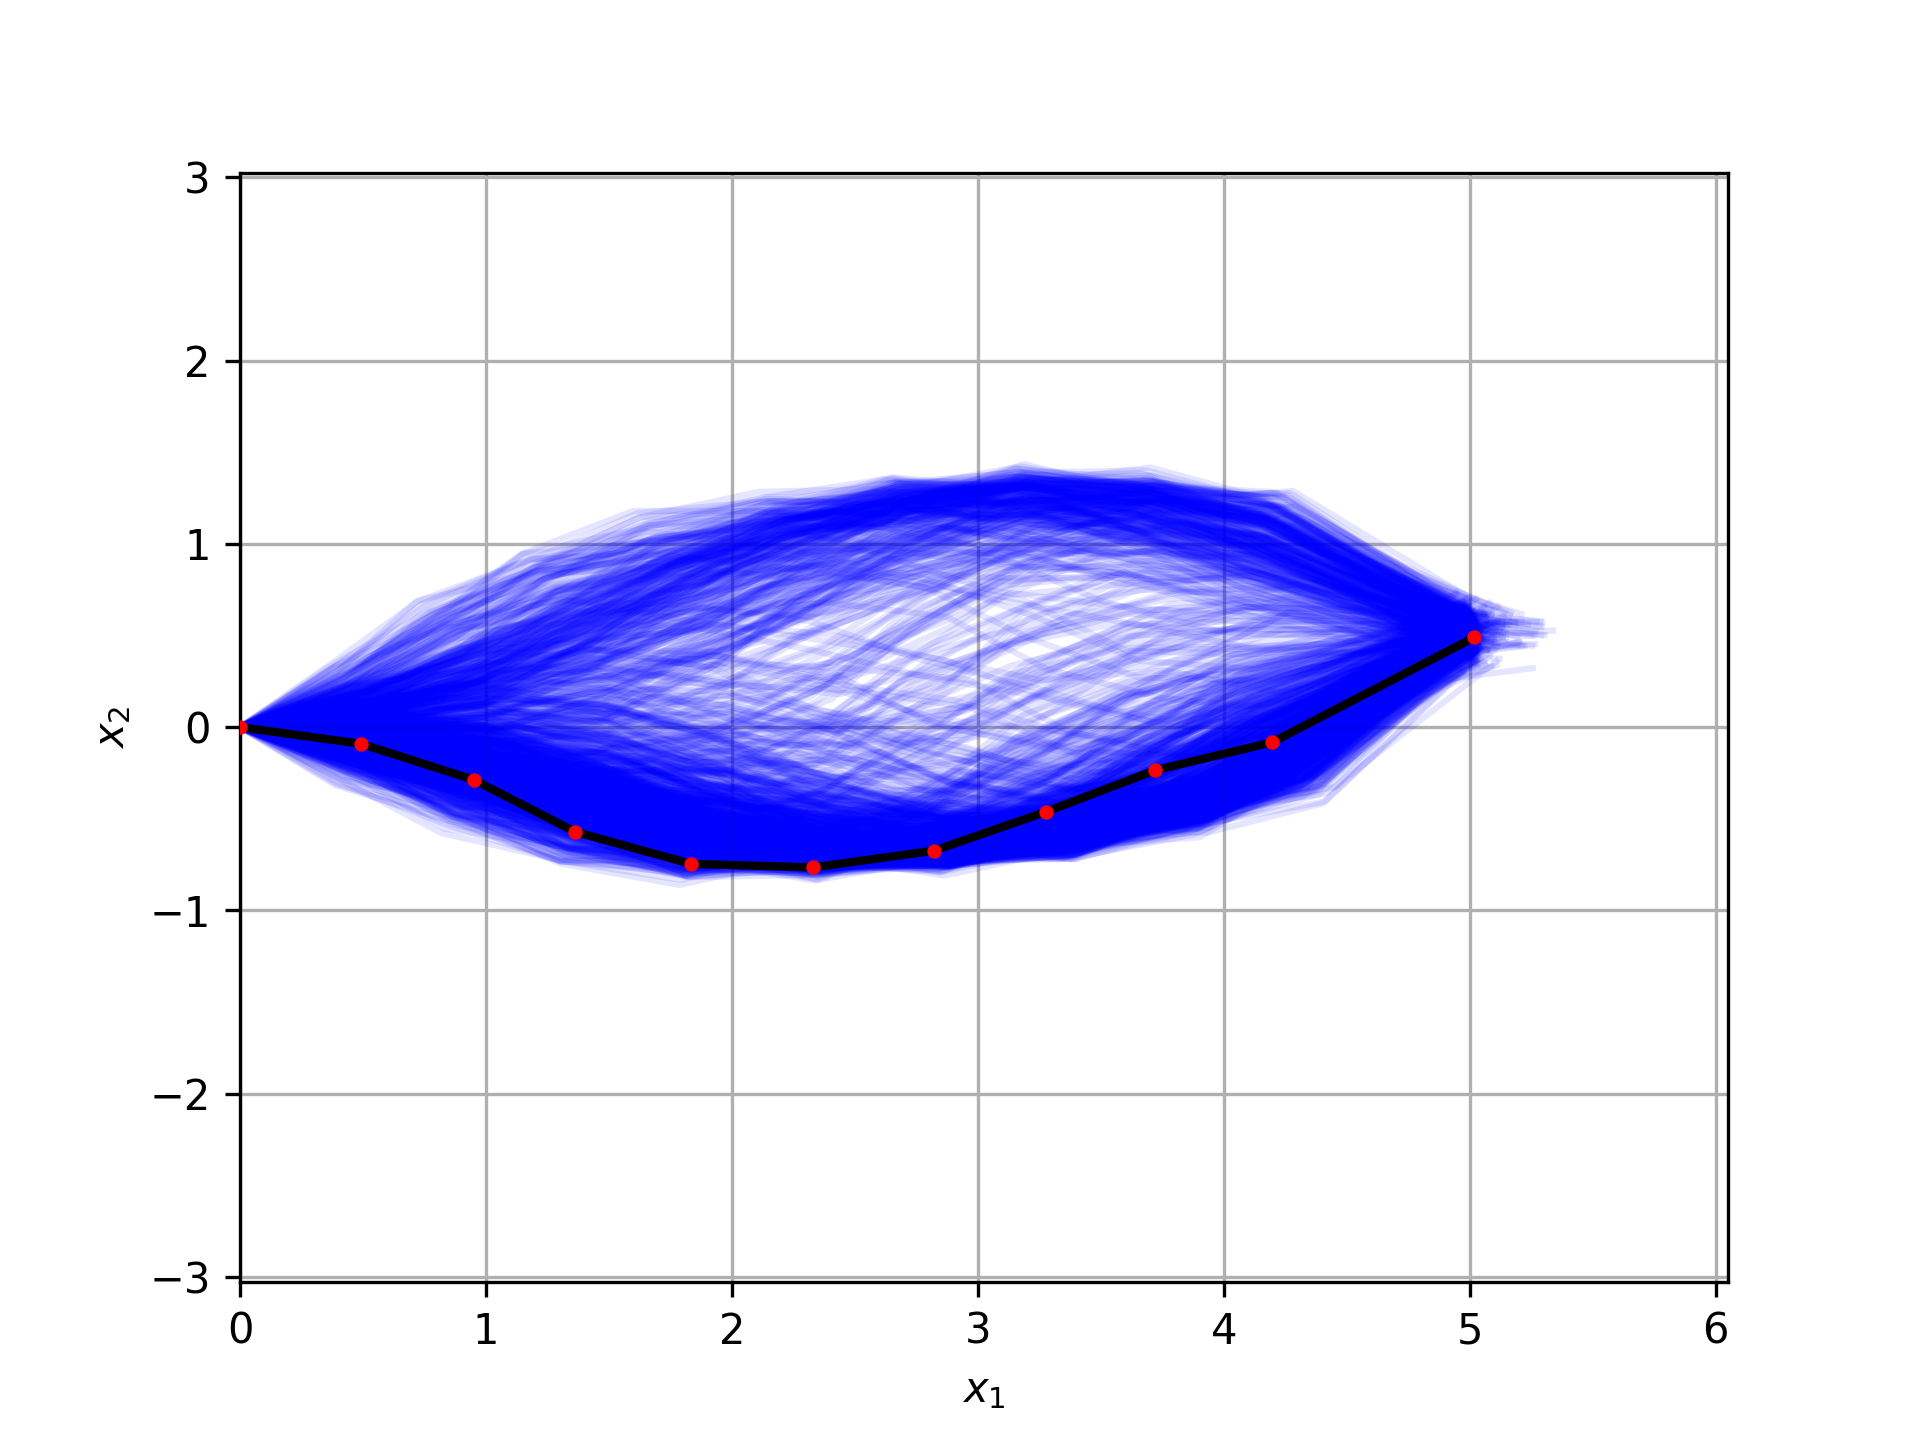
\includegraphics[width=0.29\linewidth]{figures/predicted_posterior_CVAE_10DOF.png}
        \label{fig:cVAE:10DOF}}
    %
    \subfloat[INN]{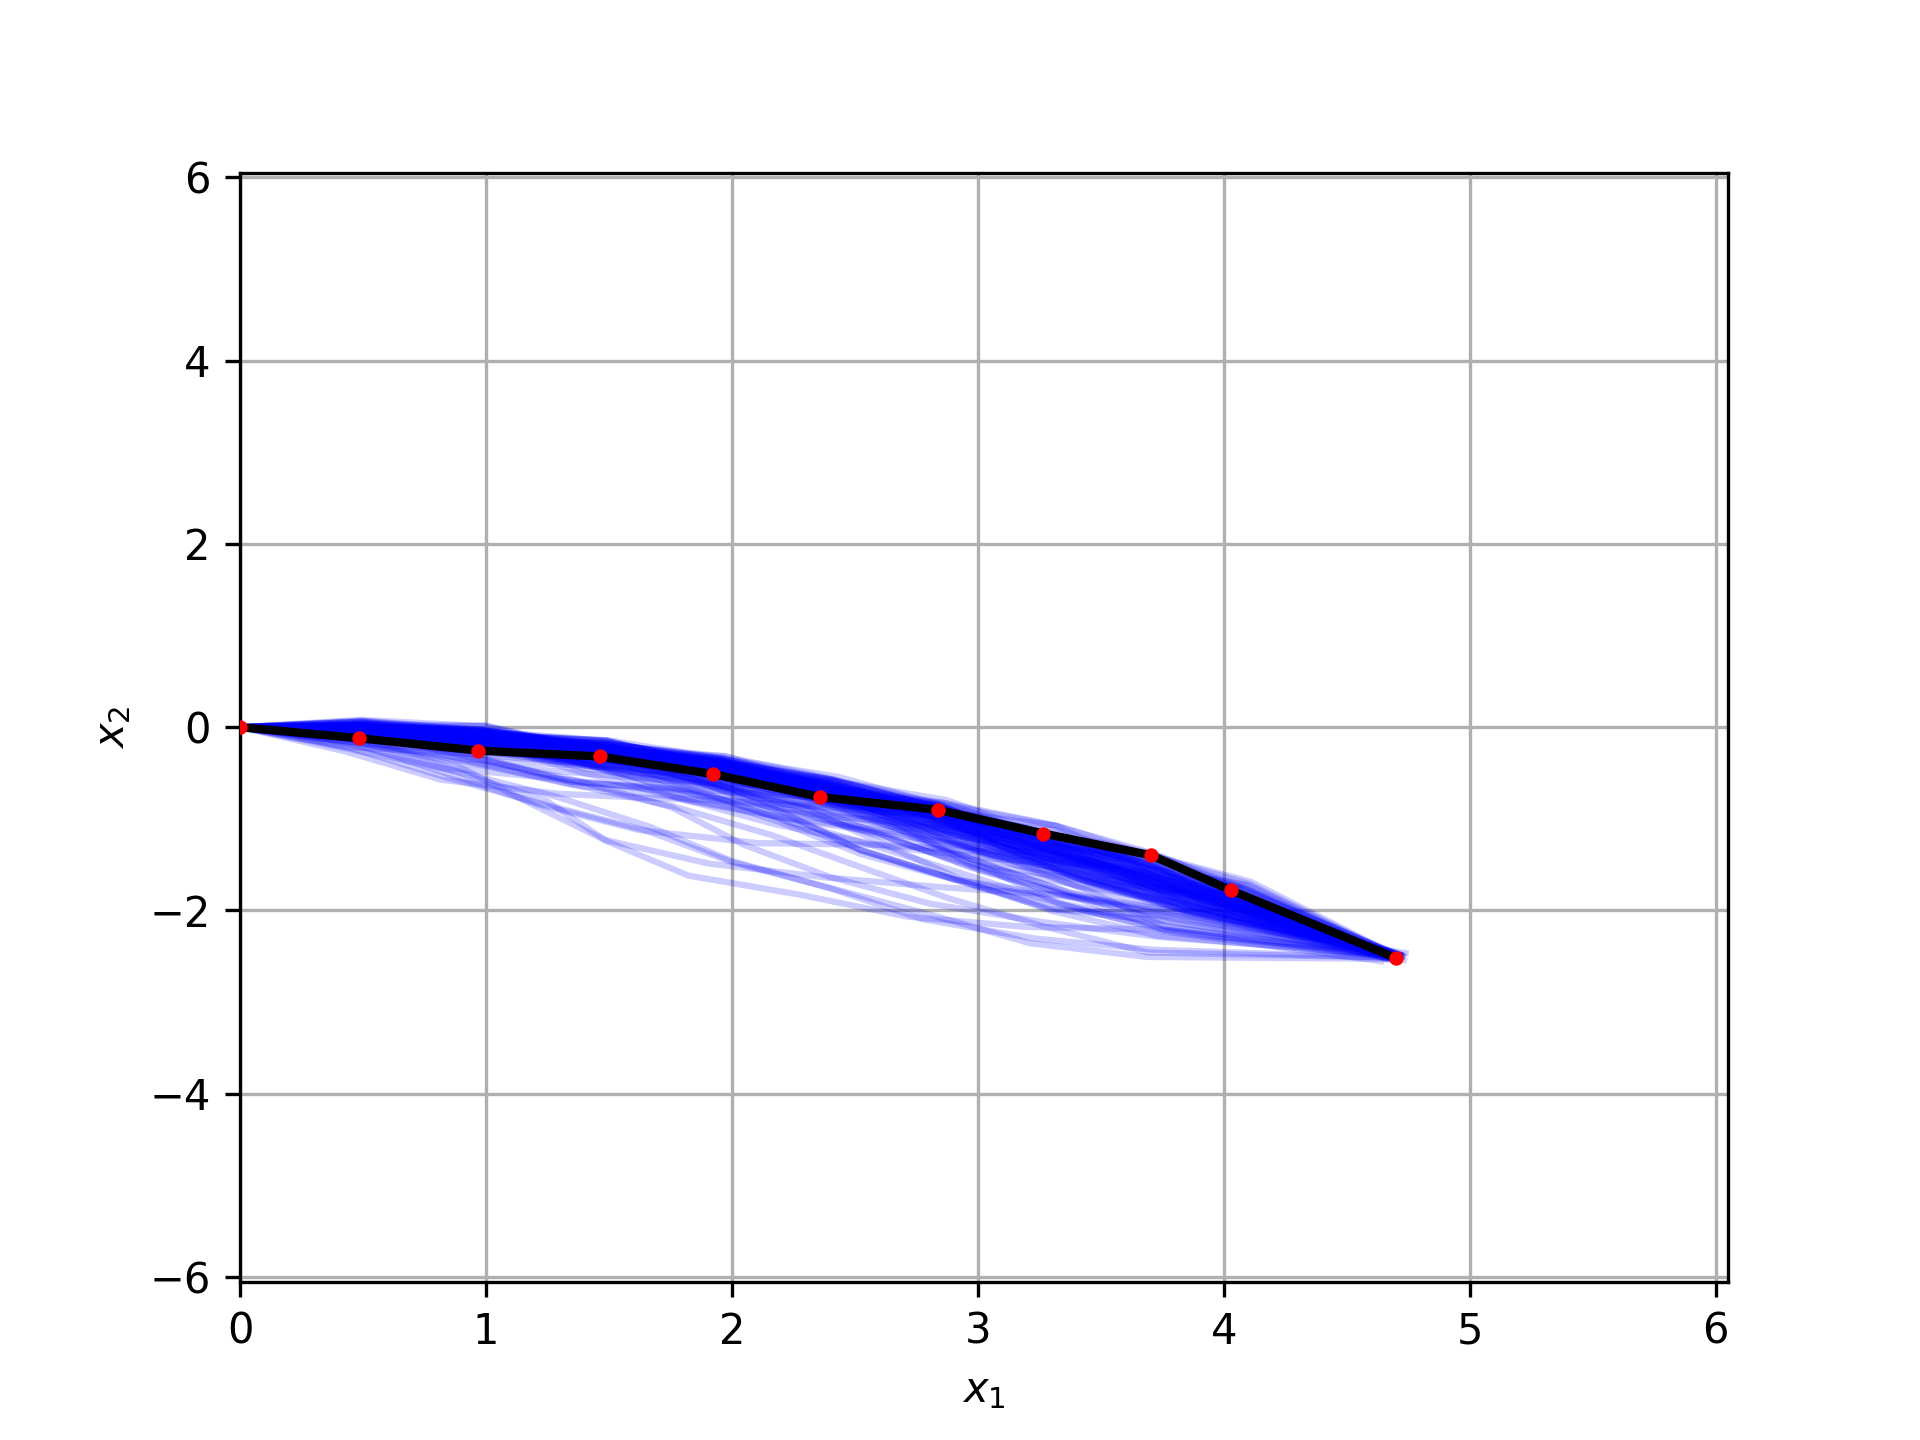
\includegraphics[width=0.29\linewidth]{figures/predicted_posterior_INN_10DOF.png}
        \label{fig:INN:10DOF}}

    \caption{\label{fig:posterior:10dof} Arm configuration of a planar manipulator with 10 revolute joints and end-effector position at $(x, y) = [4.70 -2.50]$. 100 samples are drawn from each model's predicted posterior $\tilde{p}(x | y_{gt})$, one random sample configuration is highlighted.}
\end{figure*}

\begin{figure*}[tbh]
\centering
	\subfloat[Rejection Sampling]{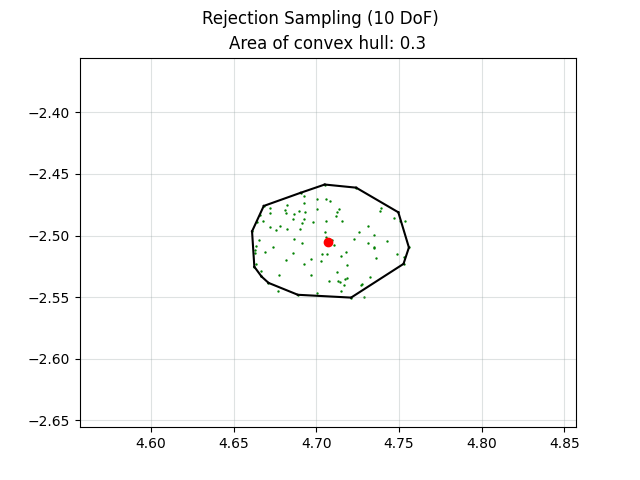
\includegraphics[width=0.45\linewidth]{figures/q_quantile_rejection_sampling_CVAE_10DOF.png}
    \label{fig:q_quantile:rejection_sampling:cVAE:10DOF}}
    %
    \subfloat[cVAE]{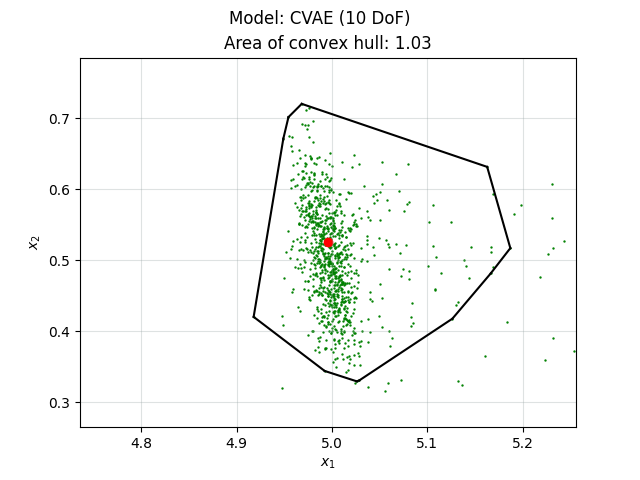
\includegraphics[width=0.45\linewidth]{figures/q_quantile_prediction_CVAE_10DOF.png}
        \label{fig:q_quantile:cVAE:10DOF}}

    \caption{\label{fig:q_quantile:cVAE:10dof} Area of the convex hull of the 0.97 percentile of the end-effector coordinates with the ground truth end-effector position at $(x, y) = [4.70 -2.50]$. Number of DoF: 10.}
\end{figure*}

\begin{figure*}[tbh]
\centering
	\subfloat[Rejection Sampling]{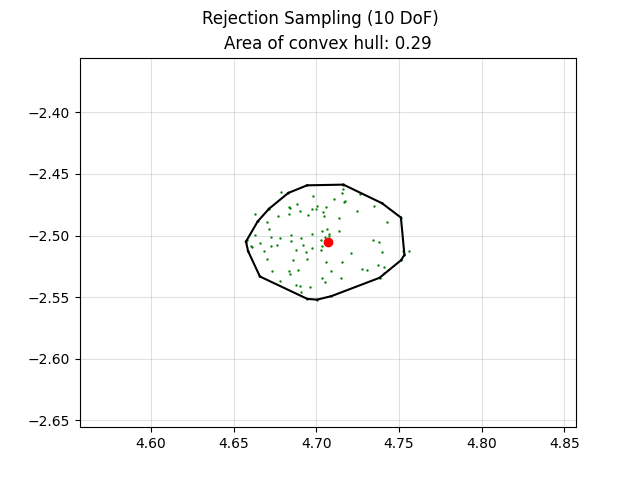
\includegraphics[width=0.45\linewidth]{figures/q_quantile_rejection_sampling_INN_10DOF.png}
    \label{fig:q_quantile:rejection_sampling:INN:10DOF}}
    %
    \subfloat[INN]{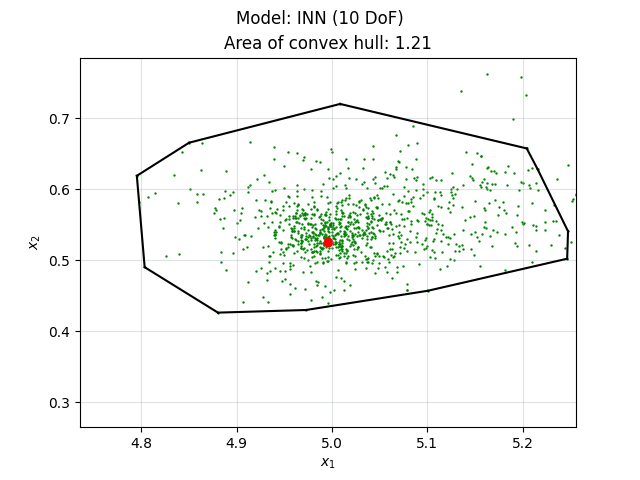
\includegraphics[width=0.45\linewidth]{figures/q_quantile_prediction_INN_10DOF.png}
        \label{fig:q_quantile:INN:10DOF}}

    \caption{\label{fig:q_quantile:INN:10dof} Area of the convex hull of the 0.97 percentile of the end-effector coordinates with the ground truth end-effector position at $(x, y) = [4.70 -2.50]$. Number of DoF: 10.}
\end{figure*}

\section*{Conclusion}


\nocite{*}
\bibliographystyle{IEEEtran}
\bibliography{IEEEabrv,final_report}

\end{document}
